\section{Warm-up: Model Checking for $\exists$-FO}\label{sec: exists FO}

\body{
    This whole section is devoted to proving the following Theorem~\ref{thm:exists-fo}. We will work with \textit{grounding} of logical formulas, that is the act of replacing quantifiers with logical connectives ranging over the entire domain. For example we will turn a formula $\exists x \exists y \phi(x,y)$ into the formula $\bigvee_{x' \in G} \bigvee_{y' \in G} \phi(x', y')$. %In other words, in the case of $\exists$-FO -- and here the distinction from full FO is important -- grounding amounts to just enumerating all possible \textit{assignments} into a structure and evaluating the remaining propositional formula. 
}

\begin{theorem}\label{thm:exists-fo}
Let $\Ta$ be a rooted binary tree co-decomposition of $\sigma$-structures with $b$ bags, each containing at most $w$ points, and let $\phi$ be an existential first-order sentence with $\ell$ variables. Letting $q=\sum_{R\in\sigma}\ell^{\operatorname{ar}(R)}$, then whether $\lim\Ta\models\phi$ can be decided, without constructing $\lim\Ta$, in time\vspace{-.5em}
\[
    \bigO{b(\ell+q)w^{2\ell}2^{2q} + w^\ell 2^q |\phi|}.\vspace{-.8em}
\]
In particular, for graphs, this gives a running time of $b\cdot 2^{\bigO{\ell^2+\ell\log(w+1)}} \operatorname{poly}(|\phi|).$ 
\end{theorem}


\begin{definition}
    Fix an ambient $\ell$-variable formula $\phi$. An \define{assignment} on a structure $G$ is a function $[\ell]\rightarrow \pts{G}$.
\end{definition}

\body{
    Since grounding the formula over the entire limit might take exponential time, we will use dynamic programming to reason about the global grounding of the formula in terms of these local assignments. To this end, we need to record not only the assignment, but also whether we already local evidence that the overall formula is false under the assignment. A canonical way of doing this is by inducing all possible relations on the points chosen by the assignment; we call these \textit{hypotheses}.
}

\begin{definition}
    Given an assignment $\beta \colon [\ell] \to \pts{G}$, denote by $\beta[G] \colon N \to G$ the unique\footnote{The structure $N$ is unique and so is the map.} homomorphism of structures -- which we call the \define{hypothesis induced on $G$ by $\beta$} -- with the following two properties: (1) the underlying function $\pts{\beta[G]} \colon \pts{N} \to \pts{G}$ is exactly the assignment $\beta$, (2) for each relation $R$ in the signature and each tuple $\vec{x}\in[\ell]^{\operatorname{ar}(R)}$, we have $R^N(\vec{x})$ if and only if $R^G(\beta(\vec{x}))$. 
\end{definition}

\body{
    As noted in Paragraph~\ref{para: bayesian}, dynamic programming over co-decompositions has a certain Bayesian feel: until one reaches the root of the co-decomposition tree, one can disprove atomic statements about the entire limit, but one can only conjecture their proofs. Hence, on their own, induced hypotheses are not enough: as we traverse the co-decomposition, we might want to remember that some relation that holds locally actually didn't hold further down the previously-explored tree. This motivates the following weaker notion.
}

\begin{definition}\label{def: hypothesis}
    A \define{hypothesis} in a structure $G$ is a homomorphism $N\xrightarrow{\nu } G$ where $\underline{N} = [\ell]$. We call $N$ the \define{head} of $\nu$ and denote it by $\text{head}(\nu)$. The \define{underlying assignment for $\nu$} is the function $\underline{\nu} \colon [\ell] \rightarrow \pts{G}$ on the sets of points. We think of a hypothesis as picking out $\ell$ points from $G$ and recording some of their relations to one another (but not necessarily all of the relational data). An induced hypothesis is a genuine induced substructure in the case where the map $\beta$ is injective. See Figure~\ref{fig:induced_env} for an example. 
\end{definition}


\body{
    We define morphisms of hypotheses below. These are important for two reasons. The first is that thinking in terms of morphisms will allow us to show that induced hypotheses satisfy a certain universal property (c.f. Proposition~\ref{prop: Universal property of induced hypotheses}) which we will use later on in proofs. The second is that morphisms of hypotheses will allow us to speak of pullbacks of hypotheses, which is the crucial ingredient towards establishing our dynamic programming algorithms both for $\exists$-FO and full FO model checking (Theorems~\ref{thm:exists-fo} and~\ref{thm: FO model checking on codecompositions}).
}

% \begin{figure}
%     \centering
%     \includegraphics[width=0.5\linewidth]{induced-env.jpg}
%     \caption{Induced hypothesis.}
%     \label{fig:induced_env}
% \end{figure}

\begin{figure}
    \begin{minipage}{0.68\textwidth}
    \includegraphics[width=0.7\linewidth, page=15]{LLJ-figs.pdf}
    \vspace{1em}
    \end{minipage}%
    \hspace{\fill}
    \begin{minipage}{0.28\textwidth}
    \caption{(Left) An assignment $\beta$ sits above a graph $G$. (Right) This induces an induced hypothesis $\beta[G]$ sitting over $G$.}
    \label{fig:induced_env}
    \end{minipage}%
\end{figure}

\vspace{-0.8em}
\begin{minipage}[t]{0.50\textwidth}
\begin{definition}\label{def: morphism of hypotheses}
    Given hypotheses $N\xrightarrow{\nu} G$ and $M\xrightarrow{\mu} H$ in structures $G$ and $H$, respectively, a \define{morphism of hypotheses} is a homomorphism $G\xrightarrow{f} H$ such that there exists a map $N\xrightarrow{q} M$ whose underlying function is $\mathsf{id}_{[\ell]}$ and which makes the diagram on the right commute.
\end{definition}
\end{minipage}
\begin{minipage}[t]{0.40\textwidth}{\small
\[\hspace{1em}\begin{tikzcd}
	{[\ell]} && {[\ell]} \\
	N && M \\
	G && H
	\arrow["{\mathsf{id}}"{description}, from=1-1, to=1-3]
	\arrow[hook, from=1-1, to=2-1]
	\arrow[hook, from=1-3, to=2-3]
	\arrow["\exists", dashed, from=2-1, to=2-3]
	\arrow["\nu"{description}, from=2-1, to=3-1]
	\arrow["\mu"{description}, from=2-3, to=3-3]
	\arrow["f"{description}, from=3-1, to=3-3]
\end{tikzcd}\]
}
\end{minipage}
\vspace{-0.3em}

\begin{lemma}\label{lemma: limits of hypotheses}
    Fix $\ell\in\mathbb{N}$. The \define{category $\mathbf{Hyp}^\sigma_{\ell}$ of $[\ell]$-hypotheses of $\sigma$-structures} is defined as follows. Its objects are hypotheses (that is, homomorphisms $\nu:N\rightarrow G$ of $\sigma$-structures such that $\pts{N}=[\ell]$) and its morphisms are given as in \cref{def: morphism of hypotheses}. Identities and composition are defined componentwise. Furthermore, the category of hypotheses and hypothesis morphisms admits pullbacks.
\end{lemma}\vspace{-.1cm}
\begin{proof}
    Verifying that $\mathbf{Hyp}^\sigma_{\ell}$ is a category is routine; we focus on proving that it admits pullbacks. The pullback of a span $(\nu:N\to G)\xrightarrow{g}(\eta:L\to K)\xleftarrow{h}(\mu:M\to H)$ of hypotheses over a span $G\xrightarrow{g}K\xleftarrow{h}H$ of structures is the map $\nu\times_\eta\mu:N\times_L M\rightarrow G\times_K H$. Viewing $\text{head}(\nu\times_\eta\mu)=N\times_L M$ again as a structure with point set $[\ell]$, we get that the pullback is again a hypothesis. In particular, a hypothesis in $G\times_K H$.
\end{proof}

\body{
    Recall that the limit of a tree co-decomposition is just an iterated pullback. Our next result shows the same is true of induced hypotheses: given an assignment to the global structure, the global\footnote{Here, and throughout, we mean ``global'' in the sense of being an assignment into the limit of the co-decompostiion.} hypothesis it induces can be recovered by taking the limit of the hypotheses induced by its projections to the bags.
}

\begin{lemma}\label{lem:lim_env_is_env_lim}
    Let $\Ta=(T,\{G_a\},\{g_t^e\})$ be a tree co-decomposition and let $\beta:[\ell]\rightarrow\pts{\lim\Ta}$ be a global assignment. Write $\beta_a$ for the projection of $\beta$ to $G_a$. Then the tuple $\Ta'=(T,\{\beta_a[G_a]\},\{g_t^e\})$ is a co-decomposition of hypotheses. Furthermore, the limit of $\Ta'$ is the hypothesis induced on the limit of $\Ta$ by $\beta$. That is, $\lim\Ta'=\beta[\lim\Ta]$. 
\end{lemma}\vspace{-.2cm}

\body{
    The universal property of pullbacks, on its own, is almost enough to prove Lemma~\ref{lem:lim_env_is_env_lim}. Indeed we require only one further universal property enojoyed by induced hypotheses. A similar universal property (c.f. Lemma~\ref{lemma: canonical comparison from projected induced to induced projected}) will be leveraged later when dealing with the case of full FO model checking. 
}

\body{
    The point of the preceding lemma is that a hypothesis on a limit is just a matching family of hypotheses in a suitably-defined co-decomposition. To make use of this, we need to project hypotheses: given a homomorphism $G\xrightarrow{\pi} H$ and a hypothesis $N\xrightarrow{\nu} G$, we call the composite $ N\xrightarrow{\pi\circ\nu} H$ the \define{projection of $\nu$ along $\pi$}. Usually $\pi$ will be the canonical projection from a (partial) limit to a bag: the resulting projection allows us to store, inside that bag, the relational information accumulated over the entire partial limit. 
}

\begin{observation}
    Notice that the projection of a hypothesis $\nu \colon N\rightarrow G$ along a map $\pi \colon G\rightarrow H$ leaves the head $N$, and hence the relations it records, unchanged. Furthermore: (1) the size of $N$ depends on the number of variables in the formula; and (2) the resulting hypothesis need not be induced (capturing the intuitive idea that, while proceeding up the tree, some relation visible locally may already have been disproved elsewhere).
\end{observation}

\begin{definition}\label{para: def: supported hypoethis}
    Now let $\Ta=(T,\{G_a\},\{g_t^e\})$ be a rooted co-decomposition (the tree $T$ has a root). For each node $i\in V(T)$, write $G[i]$ for the \define{partial limit} of $\Ta$ at $i$. That is, the limit of the tree co-decomposition obtained from $\Ta$ by restricting to the subtree rooted at $i$.
    Now fix $i$ and let $\pi_i\colon G[i]\rightarrow G_i$ be the canonical projection from the partial limit $G[i]$ to its root bag $G_i$. We say that a hypothesis $\nu_i\colon N_i\rightarrow G_i$ is \define{supported at $i$} if $\nu_i=\pi_i\circ\beta[G[i]]$ for some assignment $\beta\colon [\ell]\rightarrow\pts{G[i]}$. Given an assignment $\beta_i\colon [\ell]\rightarrow\pts{G_i}$, the \define{supported hypotheses for $\beta_i$} are those whose underlying assignment is $\beta_i$. In our analogy to Bayesian thinking: a hypothesis is supported if it has not been disproved by anything in the subtree rooted at $i$. From a dynamic programming point of view, all we need to check is the supported hypotheses at the root. \vspace{-0.1cm}
\end{definition}

\begin{lemma}\label{lemma: support at root is enough}
    Let $\phi$ be an $\ell$-variable $\exists$-FO formula, and $\Ta=(T,\{G_a\},\{g_t^e\})$ be a co-decomposition rooted at $r$. Then $\lim\Ta\models\phi$ if and only if $\operatorname{head}(\nu)\models\phi$ for some hypothesis $\nu$ supported at $r$. 
\end{lemma}
\begin{proof}
    The formula $\phi$ is satisfied in $\lim\Ta$ if and only if there is a satisfying assignment $\beta\colon [\ell]\rightarrow\pts{\lim\Ta}$. By definition, the induced hypothesis $\beta[\lim\Ta]$ records exactly the relations satisfied by the points selected by $\beta$, so $\beta$ is satisfying if and only if $\operatorname{head}(\beta[\lim\Ta])\models\phi$. Since $G[r]=\lim\Ta$, the hypotheses supported at $r$ are precisely the projections of these induced hypotheses to $G_r$. Projection leaves the head unchanged.
\end{proof}

\body{
    Lemma~\ref{lemma: support at root is enough} suggests a dynamic program. We proceed up the co-decomposition tree, starting from the leaves. To each bag $G_t$ we associate the set of supported hypotheses, and to each adhesion $G_e$ the set of hypotheses induced by assignments to $G_e$. These sets form a co-decomposition of sets, where the connecting maps send each hypothesis to the hypothesis induced by its underlying assignment on the corresponding adhesion. Matching families in this auxiliary co-decomposition are families of hypotheses whose underlying assignments agree on the adhesions. We proceed as follows. At the leaves, we simply enumerate the induced hypotheses. At internal nodes, we form matching families from the supported hypotheses of the children and induced hypotheses on the current bag. Then we combine them by taking \textit{pullbacks of hypotheses}. Finally, we project the results back to the current bag. By Lemma~\ref{lem:lim_env_is_env_lim}, we recover exactly the supported hypotheses. 
}\label{para: algorithm roadmap}

\body{
    As to the bound on the running time, note that hypotheses' heads always have precisely $\ell$ points, regardless of the size of the limit. Hence, at each node we only ever deal with at most $w^\ell 2^q$ hypotheses, where $q=\sum_{R\in\sigma}\ell^{\operatorname{ar}(R)}$. Since the algorithm considers at most pairs of such hypotheses at each node, the claimed running time follows. Finally, by Lemma~\ref{lemma: support at root is enough}, it suffices to inspect the heads of the supported hypotheses at the root to decide whether $\lim\Ta\models\phi$. The formal recurrences and their proofs are given in Section~\ref{sec: exists FO algorithms nitty-gritty}.
}

\body{
    We reiterate that the structure outlined in Paragraph~\ref{para: algorithm roadmap} is a roadmap to the case of full FO. Although the objects will be much more complicated (we will have \textit{strategies}, rather than assignments and \textit{hypotheticals}, rather than hypotheses), the algorithm is basically the same: (1) construct a co-decomposition of auxiliary data, (2) find matching families and then (3) combine these using pullbacks defined on this auxiliary data. 
}

\newpage
\subsection{Proof of Lemma~\ref{lem:lim_env_is_env_lim}}\label{sec: proof of lem:lim_env_is_env_lim}

\body{
    The proof of Lemma~\ref{lem:lim_env_is_env_lim} is straightforward, once one establishes that induced hypotheses satisfy a certain universal property (Proposition~\ref{prop: Universal property of induced hypotheses}). 
}
\begin{proposition}\label{prop: Universal property of induced hypotheses} 
    Given an assignment $\beta \colon [\ell] \to \pts{G}$, an induced hypothesis $\beta[G]$ satisfies: for any other hypothesis of the form $\gamma \colon N\to G$  with $\underline{\gamma} = \beta$, there is a unique map of hypotheses $\gamma \to \beta[G]$. %In particular, the identity on $G$.
\end{proposition}
\begin{proof}
     The unique map on the ground sets $q \colon N \to \text{head}(\beta[G])$ is fixed; we need to show it is a morphism of relational structures. Take a relation symbol $R$ and a tuple $\vec{x}$ in $N$ of the appropriate arity. By definition of morphisms of relational structures, we have that, if $R(\vec{x})$, then $R(\gamma(\vec{x}))$. But then, by definition of induced hypothesis, we have that $R(q(\vec{x}))$. Since $R$ was arbitrary $R$, we get $q$ is a morphism of structures. 
\end{proof}

\body{
    The following result states that morphisms of structures yield morphisms of induced hypotheses. We will use this result in Section~\ref{sec: exists FO} to establish Lemma~\ref{lem:lim_env_is_env_lim}, the main result in this section. In particular, we use it to prove that the tuple $\Ta'$ built from induced hypotheses is indeed a co-decomposition of hypotheses.
}

\begin{lemma}\label{lem:helper_1}
    Let $G$ and $H$ be structures and $f:G\rightarrow H$ be a homomorphism. Let $\beta:[\ell]\rightarrow \pts{G}$ be an assignment. Then $f$ is a morphism of hypotheses from $\beta[G]$ to $(f\circ\beta)[G]$.
\end{lemma}
\begin{minipage}[t]{0.45\textwidth}
    \begin{proof}
    Consider the diagram on the right. By Proposition~\ref{prop: Universal property of induced hypotheses}, and since $(f  \circ \beta)[H]$ is an induced hypothesis, there is a unique map $\text{head}(\beta[G]) \to \text{head}((f \circ \beta)[H])$ making the diagram to the right commute. 
    \end{proof}
\end{minipage}
\begin{minipage}[t]{0.45\textwidth}
\vspace{-2em}
    % https://q.uiver.app/#q=WzAsNSxbMSwyLCJHIl0sWzIsMiwiSCJdLFswLDIsIltcXGVsbF0iXSxbMSwwLCJcXHRleHR7aGVhZH0oXFxiZXRhW0ddKSJdLFsyLDAsIlxcdGV4dHtoZWFkfSgoZiBcXGNpcmMgXFxiZXRhKVtIXSkiXSxbMiwwLCJcXGJldGEiLDJdLFswLDEsImYiLDJdLFszLDAsIlxcYmV0YVtHXSJdLFs0LDEsIihmXFxjaXJjIFxcYmV0YSlbSF0iXSxbMiwzXV0=
    \[\hspace{2em}\begin{tikzcd}
	& {\text{head}(\beta[G])} & {\text{head}((f \circ \beta)[H])} \\
	\\
	{[\ell]} & G & H
	\arrow["{\beta[G]}", from=1-2, to=3-2]
	\arrow["{(f\circ \beta)[H]}", from=1-3, to=3-3]
	\arrow[from=3-1, to=1-2]
	\arrow["\beta"', from=3-1, to=3-2]
	\arrow["f"', from=3-2, to=3-3]
    \end{tikzcd}\]
    \end{minipage}

\begin{proof}[Proof of Lemma~\ref{lem:lim_env_is_env_lim}]
    For $\Ta'$ to even be well-defined, we must first check that the morphisms $g_t^e$ are morphisms of hypotheses. For every edge $e\in E(T)$ and incident node $t$, Lemma~\ref{lem:helper_1} shows that $g_t^e$ is a morphism $\beta_t[G_t]\to\beta_e[G_e]$. Thus $\Ta'$ is a co-decomposition of hypotheses.

    It remains to identify the limit of $\Ta'$. Since the limit of a tree-shaped diagram can be computed by iterated pullbacks, it suffices to prove the result for a single pullback. To that end, consider a cospan $G\xrightarrow{g}K\xleftarrow{h}H$, an assignment $\beta:[\ell]\to\pts{G\times_KH}$, and its induced hypothesis $\beta[G\times_KH]$. Write $h^\# :G\times_KH\to G$ and $g^\#:G\times_KH\to H$ for the pullback projections. By Lemma~\ref{lem:helper_1}, the following diagram commutes.
    \textbf{Note} in the rest of this proof, we use overline notation to denote the head of a hypothesis.
    
    % https://q.uiver.app/#q=WzAsOSxbMiwzLCJHIFxcdGltZXNfe0t9IEgiXSxbMCwwLCJcXG92ZXJsaW5le1xcYmV0YVtHIFxcdGltZXNfe0t9IEhdfSJdLFszLDQsIkgiXSxbNSw0LCJLIl0sWzQsMywiRyJdLFszLDIsIlxcb3ZlcmxpbmV7KGdee1xcI30gXFxjaXJjIFxcYmV0YSlbSF19Il0sWzQsMSwiXFxvdmVybGluZXsoaF57XFwjfSBcXGNpcmMgXFxiZXRhKVtHXX0iXSxbNSwyLCJcXG92ZXJsaW5leyhoIFxcY2lyYyBnXntcXCN9IFxcY2lyYyBcXGJldGEpW0tdfSJdLFsyLDEsIlxcb3ZlcmxpbmV7KGdee1xcI30gXFxjaXJjIFxcYmV0YSlbSF19IFxcdGltZXNfe1xcb3ZlcmxpbmV7KGggXFxjaXJjIGdee1xcI30gXFxjaXJjIFxcYmV0YSlbS119fSBcXG92ZXJsaW5leyhoXntcXCN9IFxcY2lyYyBcXGJldGEpW0ddfSJdLFsxLDAsIiIsMCx7ImN1cnZlIjo0fV0sWzQsMywiZyIsMV0sWzIsMywiaCIsMV0sWzAsMiwiZ157XFwjfSIsMV0sWzAsNCwiaF57XFwjfSIsMV0sWzUsMl0sWzYsNF0sWzcsM10sWzYsN10sWzUsN10sWzEsNiwiIiwwLHsiY3VydmUiOi0zfV0sWzEsNSwiIiwwLHsiY3VydmUiOjV9XSxbOCw2XSxbOCw1XV0=
\[\begin{tikzcd}[sep = small]
	{\overline{\beta[G \times_{K} H]}} &&&&& \\
	&& {\overline{(g^{\#} \circ \beta)[H]} \times_{\overline{(h \circ g^{\#} \circ \beta)[K]}} \overline{(h^{\#} \circ \beta)[G]}} && {\overline{(h^{\#} \circ \beta)[G]}} \\
	&&& {\overline{(g^{\#} \circ \beta)[H]}} && {\overline{(h \circ g^{\#} \circ \beta)[K]}} \\
	&& {G \times_{K} H} && G \\
	&&& H && K
	\arrow[curve={height=-18pt}, from=1-1, to=2-5]
	\arrow[curve={height=30pt}, from=1-1, to=3-4]
	\arrow[curve={height=24pt}, from=1-1, to=4-3]
	\arrow[from=2-3, to=2-5]
	\arrow[from=2-3, to=3-4]
	\arrow[from=2-5, to=3-6]
	\arrow[from=2-5, to=4-5]
	\arrow[from=3-4, to=3-6]
	\arrow[from=3-4, to=5-4]
	\arrow[from=3-6, to=5-6]
	\arrow["{h^{\#}}"{description}, from=4-3, to=4-5]
	\arrow["{g^{\#}}"{description}, from=4-3, to=5-4]
	\arrow["g"{description}, from=4-5, to=5-6]
	\arrow["h"{description}, from=5-4, to=5-6]
\end{tikzcd}\]
    The two morphisms from $\overline{\beta[G\times_KH]}$ to the induced hypotheses on $G$ and $H$ have the same composite with the induced hypothesis on $K$. They therefore form a cone over the pullback diagram of heads. Thus, by the universal property of this pullback, there is a unique homomorphism
    \[
    c \colon \overline{\beta[G\times_KH]} \to
    \overline{(h^\#\circ\beta)[G]} \times_{\overline{(g\circ h^\#\circ\beta)[K]}} \overline{(g^\#\circ\beta)[H]}
    \]
    making the upper triangles commute. This is shown dotted in the following diagram.
    % https://q.uiver.app/#q=WzAsOSxbMiwzLCJHIFxcdGltZXNfe0t9IEgiXSxbMCwwLCJcXG92ZXJsaW5le1xcYmV0YVtHIFxcdGltZXNfe0t9IEhdfSJdLFszLDQsIkgiXSxbNSw0LCJLIl0sWzQsMywiRyJdLFszLDIsIlxcb3ZlcmxpbmV7KGdee1xcI30gXFxjaXJjIFxcYmV0YSlbSF19Il0sWzQsMSwiXFxvdmVybGluZXsoaF57XFwjfSBcXGNpcmMgXFxiZXRhKVtHXX0iXSxbNSwyLCJcXG92ZXJsaW5leyhoIFxcY2lyYyBnXntcXCN9IFxcY2lyYyBcXGJldGEpW0tdfSJdLFsyLDEsIlxcb3ZlcmxpbmV7KGdee1xcI30gXFxjaXJjIFxcYmV0YSlbSF19IFxcdGltZXNfe1xcb3ZlcmxpbmV7KGggXFxjaXJjIGdee1xcI30gXFxjaXJjIFxcYmV0YSlbS119fSBcXG92ZXJsaW5leyhoXntcXCN9IFxcY2lyYyBcXGJldGEpW0ddfSJdLFsxLDAsIiIsMCx7ImN1cnZlIjo0fV0sWzQsMywiZyIsMV0sWzIsMywiaCIsMV0sWzAsMiwiZ157XFwjfSIsMV0sWzAsNCwiaF57XFwjfSIsMV0sWzUsMl0sWzYsNF0sWzcsM10sWzYsN10sWzUsN10sWzEsNiwiIiwwLHsiY3VydmUiOi0zfV0sWzEsNSwiIiwwLHsiY3VydmUiOjV9XSxbOCw2XSxbOCw1XSxbMSw4LCIiLDEseyJjdXJ2ZSI6LTEsInN0eWxlIjp7ImJvZHkiOnsibmFtZSI6ImRhc2hlZCJ9fX1dXQ==
\[\begin{tikzcd}[sep = small]
	{\overline{\beta[G \times_{K} H]}} &&&&& \\
	&& {\overline{(g^{\#} \circ \beta)[H]} \times_{\overline{(h \circ g^{\#} \circ \beta)[K]}} \overline{(h^{\#} \circ \beta)[G]}} && {\overline{(h^{\#} \circ \beta)[G]}} \\
	&&& {\overline{(g^{\#} \circ \beta)[H]}} && {\overline{(h \circ g^{\#} \circ \beta)[K]}} \\
	&& {G \times_{K} H} && G \\
	&&& H && K
	\arrow[curve={height=-6pt}, dashed, from=1-1, to=2-3]
	\arrow[curve={height=-18pt}, from=1-1, to=2-5]
	\arrow[curve={height=30pt}, from=1-1, to=3-4]
	\arrow[curve={height=24pt}, from=1-1, to=4-3]
	\arrow[from=2-3, to=2-5]
	\arrow[from=2-3, to=3-4]
	\arrow[from=2-5, to=3-6]
	\arrow[from=2-5, to=4-5]
	\arrow[from=3-4, to=3-6]
	\arrow[from=3-4, to=5-4]
	\arrow[from=3-6, to=5-6]
	\arrow["{h^{\#}}"{description}, from=4-3, to=4-5]
	\arrow["{g^{\#}}"{description}, from=4-3, to=5-4]
	\arrow["g"{description}, from=4-5, to=5-6]
	\arrow["h"{description}, from=5-4, to=5-6]
\end{tikzcd}\]
    By Lemma~\ref{lemma: limits of hypotheses}, the pullback of the two induced hypotheses over the induced hypothesis on $K$ is itself a hypothesis $\overline{(h^\#\circ\beta)[G]} \times_{\overline{(g\circ h^\#\circ\beta)[K]}} \overline{(g^\#\circ\beta)[H]}
    \to G\times_KH$; this is the red, dashed arrow below.
   % https://q.uiver.app/#q=WzAsOSxbMiwzLCJHIFxcdGltZXNfe0t9IEgiXSxbMCwwLCJcXG92ZXJsaW5leyhHIFxcdGltZXNfe0t9IEgpW1xcYmV0YV19Il0sWzMsNCwiSCJdLFs1LDQsIksiXSxbNCwzLCJHIl0sWzMsMiwiXFxvdmVybGluZXtIW2dee1xcI30gXFxjaXJjIFxcYmV0YV19Il0sWzQsMSwiXFxvdmVybGluZXtHW2hee1xcI30gXFxjaXJjIFxcYmV0YV19Il0sWzUsMiwiS1toIFxcY2lyYyBnXntcXCN9IFxcY2lyYyBcXGJldGFdIl0sWzIsMSwiXFxvdmVybGluZXtIW2dee1xcI30gXFxjaXJjIFxcYmV0YV19IFxcdGltZXNfe1xcb3ZlcmxpbmV7S1toIFxcY2lyYyBnXntcXCN9IFxcY2lyYyBcXGJldGFdfX0gXFxvdmVybGluZXtHW2hee1xcI30gXFxjaXJjIFxcYmV0YV19Il0sWzEsMCwiIiwwLHsiY3VydmUiOjR9XSxbNCwzLCJnIiwxXSxbMiwzLCJoIiwxXSxbMCwyLCJnXntcXCN9IiwxXSxbMCw0LCJoXntcXCN9IiwxXSxbNSwyXSxbNiw0XSxbNywzXSxbNiw3XSxbNSw3XSxbMSw2LCIiLDAseyJjdXJ2ZSI6LTN9XSxbMSw1LCIiLDAseyJjdXJ2ZSI6NX1dLFs4LDZdLFs4LDVdLFsxLDgsIiIsMSx7ImN1cnZlIjotMSwic3R5bGUiOnsiYm9keSI6eyJuYW1lIjoiZGFzaGVkIn19fV0sWzgsMCwiIiwxLHsiY29sb3VyIjpbMCw2MCw2MF0sInN0eWxlIjp7ImJvZHkiOnsibmFtZSI6ImRhc2hlZCJ9fX1dXQ==
\[\begin{tikzcd}[row sep=small]
	{\overline{(G \times_{K} H)[\beta]}} &&&&& \\
	&& {\overline{H[g^{\#} \circ \beta]} \times_{\overline{K[h \circ g^{\#} \circ \beta]}} \overline{G[h^{\#} \circ \beta]}} && {\overline{G[h^{\#} \circ \beta]}} \\
	&&& {\overline{H[g^{\#} \circ \beta]}} && {K[h \circ g^{\#} \circ \beta]} \\
	&& {G \times_{K} H} && G \\
	&&& H && K
	\arrow[curve={height=-6pt}, dashed, from=1-1, to=2-3]
	\arrow[curve={height=-18pt}, from=1-1, to=2-5]
	\arrow[curve={height=30pt}, from=1-1, to=3-4]
	\arrow[curve={height=24pt}, from=1-1, to=4-3]
	\arrow[from=2-3, to=2-5]
	\arrow[from=2-3, to=3-4]
	\arrow[draw={rgb,255:red,214;green,92;blue,92}, dashed, from=2-3, to=4-3]
	\arrow[from=2-5, to=3-6]
	\arrow[from=2-5, to=4-5]
	\arrow[from=3-4, to=3-6]
	\arrow[from=3-4, to=5-4]
	\arrow[from=3-6, to=5-6]
	\arrow["{h^{\#}}"{description}, from=4-3, to=4-5]
	\arrow["{g^{\#}}"{description}, from=4-3, to=5-4]
	\arrow["g"{description}, from=4-5, to=5-6]
	\arrow["h"{description}, from=5-4, to=5-6]
\end{tikzcd}\]
    By Proposition~\ref{prop: Universal property of induced hypotheses}, the existence of the red dashed arrow implies the existence of the arrow $q$ below (depicted in blue below).
   % https://q.uiver.app/#q=WzAsOSxbMiwzLCJHIFxcdGltZXNfe0t9IEgiXSxbMCwwLCJcXG92ZXJsaW5le1xcYmV0YVtHIFxcdGltZXNfe0t9IEhdfSJdLFszLDQsIkgiXSxbNSw0LCJLIl0sWzQsMywiRyJdLFszLDIsIlxcb3ZlcmxpbmV7KGdee1xcI30gXFxjaXJjIFxcYmV0YSlbSF19Il0sWzQsMSwiXFxvdmVybGluZXsoaF57XFwjfSBcXGNpcmMgXFxiZXRhKVtHXX0iXSxbNSwyLCJcXG92ZXJsaW5leyhoIFxcY2lyYyBnXntcXCN9IFxcY2lyYyBcXGJldGEpW0tdfSJdLFsyLDEsIlxcb3ZlcmxpbmV7KGdee1xcI30gXFxjaXJjIFxcYmV0YSlbSF19IFxcdGltZXNfe1xcb3ZlcmxpbmV7KGggXFxjaXJjIGdee1xcI30gXFxjaXJjIFxcYmV0YSlbS119fSBcXG92ZXJsaW5leyhoXntcXCN9IFxcY2lyYyBcXGJldGEpW0ddfSJdLFsxLDAsIiIsMCx7ImN1cnZlIjo0fV0sWzQsMywiZyIsMV0sWzIsMywiaCIsMV0sWzAsMiwiZ157XFwjfSIsMV0sWzAsNCwiaF57XFwjfSIsMV0sWzUsMl0sWzYsNF0sWzcsM10sWzYsN10sWzUsN10sWzEsNiwiIiwwLHsiY3VydmUiOi0zfV0sWzEsNSwiIiwwLHsiY3VydmUiOjV9XSxbOCw2XSxbOCw1XSxbMSw4LCJjIiwxLHsiY3VydmUiOi0xLCJzdHlsZSI6eyJib2R5Ijp7Im5hbWUiOiJkYXNoZWQifX19XSxbOCwwLCIiLDEseyJjb2xvdXIiOlswLDYwLDYwXSwic3R5bGUiOnsiYm9keSI6eyJuYW1lIjoiZGFzaGVkIn19fV0sWzgsMSwicSIsMSx7ImxhYmVsX3Bvc2l0aW9uIjo4MCwiY3VydmUiOi0xLCJjb2xvdXIiOlsyMzgsNzcsNjBdLCJzdHlsZSI6eyJib2R5Ijp7Im5hbWUiOiJkb3R0ZWQifX19XV0=
\[\begin{tikzcd}[sep = small]
	{\overline{\beta[G \times_{K} H]}} &&&&& \\
	&& {\overline{(g^{\#} \circ \beta)[H]} \times_{\overline{(h \circ g^{\#} \circ \beta)[K]}} \overline{(h^{\#} \circ \beta)[G]}} && {\overline{(h^{\#} \circ \beta)[G]}} \\
	&&& {\overline{(g^{\#} \circ \beta)[H]}} && {\overline{(h \circ g^{\#} \circ \beta)[K]}} \\
	&& {G \times_{K} H} && G \\
	&&& H && K
	\arrow["c"{description}, curve={height=-6pt}, dashed, from=1-1, to=2-3]
	\arrow[curve={height=-18pt}, from=1-1, to=2-5]
	\arrow[curve={height=30pt}, from=1-1, to=3-4]
	\arrow[curve={height=24pt}, from=1-1, to=4-3]
	\arrow["q"{description, pos=0.8}, draw={rgb,255:red,74;green,80;blue,232}, curve={height=-6pt}, dotted, from=2-3, to=1-1]
	\arrow[from=2-3, to=2-5]
	\arrow[from=2-3, to=3-4]
	\arrow[draw={rgb,255:red,214;green,92;blue,92}, dashed, from=2-3, to=4-3]
	\arrow[from=2-5, to=3-6]
	\arrow[from=2-5, to=4-5]
	\arrow[from=3-4, to=3-6]
	\arrow[from=3-4, to=5-4]
	\arrow[from=3-6, to=5-6]
	\arrow["{h^{\#}}"{description}, from=4-3, to=4-5]
	\arrow["{g^{\#}}"{description}, from=4-3, to=5-4]
	\arrow["g"{description}, from=4-5, to=5-6]
	\arrow["h"{description}, from=5-4, to=5-6]
\end{tikzcd}\]
    It remains to check that $c$ and $q$ are inverse. Under the canonical identification of both point sets with $[\ell]$, the underlying functions of $c$ and $q$ are both $\mathsf{id}_{[\ell]}$. Hence the underlying functions of $q\circ c$ and $c\circ q$ are identity functions. Since homomorphisms of relational structures are determined by their underlying functions, this implies that $\beta[G\times_KH] \cong (h^\#\circ\beta)[G] \times_{(g\circ h^\#\circ\beta)[K]} (g^\#\circ\beta)[H].$
\end{proof}

\subsection{Computing Supported Hypotheses by Dynamic Programming}\label{sec: exists FO algorithms nitty-gritty}

\body{
    It remains to show how to efficiently calculate the supported hypotheses at a given bag. To that end, given a rooted tree co-decomposition $\Ta$ and any node $t$ therein, denote by $H(t)$ the set of hypotheses on $G_t$ and by $\Ha_{supp}(t) := \{\nu \colon N \to G_t \mid \nu \text{ is a supported hypothesis at } t\}$ the set of supported hypotheses at $t$. 
}\label{para: set of supported hypotheses for dyn prog}

\begin{lemma}
    Let $\Ta$ be a rooted tree co-decomposition and let $i$ denote a leaf node without children. For an assignment $\beta_i$ to $G_i$, there is a single supported hypothesis for $\beta_i$, namely the induced hypothesis $\beta_i[G_i]$. Consequently $H(i) = \Ha_{supp}(i)$.
\end{lemma}
\begin{proof}
    The partial limit $G[i]$ at $i$ is identical to $G_i$.
\end{proof}

\begin{lemma}\label{lem:running_env}
Let $\Ta$ be a rooted tree co-decomposition, let $t$ be a node with unique child $c$, and write $e=ct$. Let $p_t\colon G_c\times_{G_e}G_t\rightarrow G_t$ be the pullback projection. Then $\Ha_{\mathrm{supp}}(t)$ can be computed from $\Ha_{\mathrm{supp}}(c)$ as follows. For $\rho\in\Ha_{\mathrm{supp}}(c)$, write $\beta_c$ for its underlying assignment. An assignment $\beta_t$ to $G_t$ is \define{compatible with $\rho$} if $g_c^e\circ\beta_c=g_t^e\circ\beta_t$. For such a compatible pair, write $\beta_e$ for this common assignment to $G_e$. Then\vspace{-.5em}
\[
\Ha_{\mathrm{supp}}(t)
=
\left\{
p_t\circ
\left(
\rho\times_{\beta_e[G_e]}\beta_t[G_t]
\right)
\;\middle|\;
\rho\in\Ha_{\mathrm{supp}}(c)
\text{ and }
\beta_t\text{ is compatible with }\rho
\right\}.
\]
\end{lemma}

\begin{proof}
To help keep track of variables, we will use hats on assignments and hypotheses on the partial limit.
Let $\rho\in\Ha_{\mathrm{supp}}(c)$ and let $\beta_t$ be compatible with $\rho$. Since $\rho$ is supported, there is an assignment $\widehat{\beta}_c\colon[\ell]\rightarrow\pts{G[c]}$ such that the induced hypothesis $\widehat{\rho}:=\widehat{\beta}_c[G[c]]$ projects to $\rho$. The assignments $\widehat{\beta}_c$ and $\beta_t$ agree on $G_e$, so they determine an assignment $\beta$ to $G[t]=G[c]\times_{G_e}G_t$. By Lemma~\ref{lem:lim_env_is_env_lim}, the hypothesis induced by $\beta$ on $G[t]$ is $\widehat{\rho}\times_{\beta_e[G_e]}\beta_t[G_t]$.

Consider also the pullback $\rho\times_{\beta_e[G_e]}\beta_t[G_t]$. Since projection leaves the head unchanged, $\widehat{\rho}$ and $\rho$ have the same head, and the two pullbacks also have the same head. For readability in the diagram, write $R$ for the common head of $\widehat{\rho}$ and $\rho$, write $I=\operatorname{head}(\beta_t[G_t])$ and $K=\operatorname{head}(\beta_e[G_e])$, and write $S$ for the common head of the two pullbacks. The canonical projection ${\color{red}q}\colon G[t]\rightarrow G_c\times_{G_e}G_t$ then makes the following diagram commute. \vspace{-0.5em}
\[
\begin{tikzcd}[row sep=small]
	&&&& S \\
	R &&&& {G[t]=G[c]\times_{G_e}G_t} \\
	{G[c]} && S \\
	R && {G_c\times_{G_e}G_t} && I \\
	{G_c} && K && {G_t} \\
	&& {G_e}
	\arrow["{\widehat{\rho}\times_{\beta_e[G_e]}\beta_t[G_t]}", from=1-5, to=2-5]
	\arrow["{\mathrm{id}_S}"', dashed, from=1-5, to=3-3]
	\arrow["{\widehat{\rho}}", from=2-1, to=3-1]
	\arrow["{\mathrm{id}_R}"', curve={height=18pt}, dashed, from=2-1, to=4-1]
	\arrow[from=2-5, to=3-1]
	\arrow["q", dashed, from=2-5, to=4-3, color=red]
	\arrow[curve={height=-30pt}, from=2-5, to=5-5]
	\arrow[curve={height=12pt}, from=3-1, to=5-1]
	\arrow["{\rho\times_{\beta_e[G_e]}\beta_t[G_t]}"', from=3-3, to=4-3]
	\arrow["\rho", from=4-1, to=5-1]
	\arrow[from=4-3, to=5-1]
	\arrow[from=4-3, to=5-5]
	\arrow["{\beta_t[G_t]}"', from=4-5, to=5-5]
	\arrow["{g_c^e}"', from=5-1, to=6-3]
	\arrow["{\beta_e[G_e]}"', from=5-3, to=6-3]
	\arrow["{g_t^e}", from=5-5, to=6-3]
\end{tikzcd}
\]

Thus $\rho\times_{\beta_e[G_e]}\beta_t[G_t]$ is the projection of the induced hypothesis $\widehat{\rho}\times_{\beta_e[G_e]}\beta_t[G_t]$ along $q$. It follows that $p_t\circ(\rho\times_{\beta_e[G_e]}\beta_t[G_t])$ is its projection to $G_t$, and hence belongs to $\Ha_{\mathrm{supp}}(t)$.

Conversely, let $\nu\in\Ha_{\mathrm{supp}}(t)$. By supportedness, $\nu$ is the projection to $G_t$ of $\beta[G[t]]$ for some assignment $\beta$ to $G[t]$. Let $\widehat{\beta}_c$ and $\beta_t$ be the projections of $\beta$ to $G[c]$ and $G_t$, respectively. Let $\widehat{\rho}=\widehat{\beta}_c[G[c]]$, and $\rho$ be the projection of $\widehat{\rho}$ to $G_c$. Then $\rho\in\Ha_{\mathrm{supp}}(c)$ and $\beta_t$ is compatible with $\rho$. By Lemma~\ref{lem:lim_env_is_env_lim}, the hypothesis $\beta[G[t]]$ is $\widehat{\rho}\times_{\beta_e[G_e]}\beta_t[G_t]$. The preceding diagram therefore gives $\nu=p_t\circ(\rho\times_{\beta_e[G_e]}\beta_t[G_t])$, as required.
\end{proof}

In the following, each $\nu_j\rightarrow\beta_t[G_t]$ is the canonical morphism to the induced hypothesis for its underlying assignment, and we use the canonical identification $G_t\times_{G_t}G_t\cong G_t$.
\begin{lemma}\label{lem:two_children}
Let $\Ta$ be a rooted tree co-decomposition and let $t$ be a node with exactly two children $c_1$ and $c_2$. For each $j\in\{1,2\}$, apply Lemma~\ref{lem:running_env} as if $c_j$ were the unique child of $t$, and denote the resulting set of hypotheses on $G_t$ by $\Ha_{c_j\to t}$. Then\vspace{-.5em}
\[
\Ha_{\mathrm{supp}}(t)
=
\left\{
\nu_1\times_{\beta_t[G_t]}\nu_2
\;\middle|\;
\nu_j\in\Ha_{c_j\to t}\text{ for }j\in\{1,2\},
\text{ and }\nu_1,\nu_2
\text{ have underlying assignment }\beta_t
\right\}.\vspace{-.5em}
\]
That is, $\Ha_{\mathrm{supp}}(t)$ is obtained by taking pairwise pullbacks of hypotheses in $\Ha_{c_1\to t}$ and $\Ha_{c_2\to t}$ with the same underlying assignment.
\end{lemma}
\begin{proof}
For $j\in\{1,2\}$, let $\Ta_j$ be the co-decomposition obtained by restricting $\Ta$ to $t$ and the subtree rooted at $c_j$, and write $G_j[t]$ for its limit. Thus $G[t]\cong G_1[t]\times_{G_t}G_2[t]$.

First, let $\nu_j\in\Ha_{c_j\to t}$ for $j\in\{1,2\}$, and suppose that both have underlying assignment $\beta_t$. Since $\nu_j$ is supported with respect to $\Ta_j$, there is an assignment $\widehat{\beta}_j\colon[\ell]\rightarrow\pts{G_j[t]}$ such that the induced hypothesis $\widehat{\nu}_j:=\widehat{\beta}_j[G_j[t]]$ projects to $\nu_j$. The assignments $\widehat{\beta}_1$ and $\widehat{\beta}_2$ agree on $G_t$, since both project to $\beta_t$, and therefore determine an assignment $\beta$ to $G[t]$.

By Lemma~\ref{lem:lim_env_is_env_lim}, the hypothesis induced by $\beta$ is $\widehat{\nu}_1\times_{\beta_t[G_t]}\widehat{\nu}_2$. By the universal property of pullbacks, its projection to $G_t$ is $\nu_1\times_{\beta_t[G_t]}\nu_2$. Hence this hypothesis belongs to $\Ha_{\mathrm{supp}}(t)$.

Conversely, let $\nu\in\Ha_{\mathrm{supp}}(t)$, witnessed by an assignment $\beta\colon[\ell]\rightarrow\pts{G[t]}$. For each $j\in\{1,2\}$, project $\beta$ to an assignment $\widehat{\beta}_j$ on $G_j[t]$, let $\widehat{\nu}_j=\widehat{\beta}_j[G_j[t]]$, and let $\nu_j$ be its projection to $G_t$. Then $\nu_j\in\Ha_{c_j\to t}$, and both $\nu_1$ and $\nu_2$ have the same underlying assignment $\beta_t$, namely the projection of $\beta$ to $G_t$. Applying Lemma~\ref{lem:lim_env_is_env_lim} and projecting to $G_t$ gives $\nu=\nu_1\times_{\beta_t[G_t]}\nu_2$, as required.
\end{proof}

\begin{proof}[Proof of Theorem~\ref{thm:exists-fo}]
Note that a hypothesis with underlying assignment $\beta \colon [\ell]\to\pts{G_t}$ is determined by which of the $q : =\sum_{R\in\sigma}\ell^{\operatorname{ar}(R)}$ possible atomic relations on $[\ell]$ hold in its head. Thus, since each bag has at most $w$ points, there are at most $w^\ell 2^q$ hypotheses on any given bag.

With this in mind, process the nodes of $T$ from the leaves towards the root. At a leaf $t$, the supported hypotheses are precisely the induced hypotheses $\beta_t[G_t]$. If $t$ has one child, compute the supported hypotheses $\Ha_{\mathrm{supp}}(t)$ from those of its child using Lemma~\ref{lem:running_env}. If $t$ has two children, first perform the single-child computation separately for each child and then combine the resulting sets using Lemma~\ref{lem:two_children}. Since $T$ is binary, these are all the possible cases. At a node with one child, we consider at most $w^{2\ell}2^q$ compatible pairs of hypotheses and assignments. At a node with two children, we additionally consider at most $w^{2\ell}2^{2q}$ pairs of hypotheses. Checking compatibility and computing pullbacks of hypotheses takes $O(\ell+q)$ time, since their heads have only $\ell$ points. Thus, the total time required to compute all supported-hypothesis tables is $O\left(b(\ell+q)w^{2\ell}2^{2q}\right)$. Finally, at the root $r$, we evaluate the quantifier-free part of $\phi$ on the distinguished variables of each head of a supported hypothesis. Since there are at most $w^\ell 2^q$ such hypotheses, this requires an additional $O(w^\ell 2^q|\phi|)$ time. By Lemma~\ref{lemma: support at root is enough}, this decides whether $\lim\Ta\models\phi$, giving the claimed running time $O\left( b(\ell+q)w^{2\ell}2^{2q} +w^\ell 2^q|\phi| \right).$ 
\end{proof}

